\documentclass[a5paper, twoside]{article}  %online/print need to use same page size 
\setcounter{secnumdepth}{5}
\setcounter{tocdepth}{5}
\usepackage[english]{babel}
\usepackage{textcomp}
\usepackage{amsmath,amsthm,amsfonts,amssymb,epsfig}
\usepackage{array}
\usepackage{datetime}
\usepackage{lipsum}% http://ctan.org/pkg/lipsum
\usepackage[total={5.4in,8.4in},top=1in, left=0.5in, right=0.5in, bottom=1in]{geometry}
\usepackage{listings}% http://ctan.org/pkg/listings
\usepackage{spverbatim}
\usepackage[hidelinks]{hyperref}
\Urlmuskip=0mu plus 1mu\relax %needed to make long URLs break nicely
\usepackage{microtype}
\hypersetup{colorlinks=false}
\usepackage{graphicx}
\graphicspath{ {images/} }
\usepackage{parskip}
\usepackage{titlesec} %used for diminishing heading sizes
\titleformat{\section}{\normalfont\bfseries}{\thesection}{1em}{}
\titlespacing*{\section}{0pt}{*2}{0pt}
\titlespacing*{\subsection}{0pt}{*2}{0pt}
\usepackage[square, sort, comma, numbers]{natbib} %%uses titles for cited references
\usepackage[fit]{truncate}
\usepackage{fancyhdr}
\pagestyle{fancy}
\renewcommand{\sectionmark}[1]{\markboth{#1}{}}
\fancyhead{}
\fancyhead[OR]{\leftmark \hspace{0.1cm}  $\vert$ \hspace{0.1cm}  \thepage}
\fancyhead[EL]{\thepage \hspace{0.1cm} $\vert$ \hspace{0.1cm} \leftmark}
\fancyfoot[C]{}%hide footer 
\usepackage{xcolor} 
\usepackage[scaled=1]{couriers}
\xdefinecolor{gray}{rgb}{0.6,0.6,0.6} 
\usepackage{setspace}
\usepackage{adjustbox}


\input{common/conf_titles.tex}
%
% Use fancy table
%
\usepackage{tabularx}
\usepackage{booktabs}

\begin{document}


%----------------------------------------------------------------------
% Definition for "lstlisting" blocks
%----------------------------------------------------------------------
% --- USAGE ---
%
% \begin{lstlisting}[style=R}
% ...
% \end{lstlisting}
%
% % \begin{lstlisting}[style=output}
% ...
% \end{lstlisting}
%----------------------------------------------------------------------

% By default, make listings all black so it's easy to spot the ones that aren't set to a style.
% This is just a debugging technique.
\lstset{backgroundcolor=\color{black}}

\lstdefinestyle{R}{
  language=R,
  frame=single,
  breaklines,
  basicstyle=\ttfamily,
  commentstyle=\textbf,% comment style
  keywordstyle=\ttfamily,
  numbers=left,% display line numbers on the left side 
  numberstyle=\scriptsize,% use small line numbers 
  numbersep=10pt,% space between line numbers and code
  backgroundcolor=\color{white}
}

\lstdefinestyle{python}{
  language=python,
  frame=single,
  breaklines,
  basicstyle=\ttfamily,
  commentstyle=\textsl,% comment style
  keywordstyle=\ttfamily,
  numbers=left,% display line numbers on the left side 
  numberstyle=\scriptsize,% use small line numbers 
  numbersep=10pt,% space between line numbers and code
  backgroundcolor=\color{white}
}

\definecolor{mygray}{rgb}{0.92,0.92,0.92}

\lstdefinestyle{output}{
  frame=single,
  breaklines,
  basicstyle=\ttfamily,
  numbers=left,% display line numbers on the left side 
  numberstyle=\scriptsize,% use small line numbers 
  numbersep=10pt,% space between line numbers and code
  backgroundcolor=\color{mygray}
}

\newcommand{\waterExampleInR} {
\textbf{Example in R} \\
}

\newcommand{\waterExampleInPython} {
\textbf{Example in Python} \\
}


\thispagestyle{empty} %removes page number  

\begin{center}
\textsc{\Large\bf{Sparkling Water}}
\\
\bigskip
\textsc{\small{Michal Malohlava\hspace{40pt} Alex Tellez \hspace{40pt} Jessica Lanford}}
\\
\bigskip
\line(1,0){250}  %inserts  horizontal line


{\url{http://h2o.gitbooks.io/sparkling-water-and-h2o/}}

\bigskip
August 2015: First Edition 
\\%add front page image here? (wavy lines)
\bigskip
\end{center}

{\raggedright\vfill\ 

Sparkling Water\\
  by Michal Malohlava, Alex Tellez \&\ Jessica Lanford\\
\bigskip
  Published by H2O.ai, Inc. \\
2307 Leghorn St. \\
Mountain View, CA 94043\\
\bigskip
\textcopyright 2015 H2O.ai, Inc. All Rights Reserved. 
\bigskip

August 2015: First Edition
\bigskip

Photos by \textcopyright H2O.ai, Inc. 
\bigskip

While every precaution has been taken in the\\
preparation of this book, the publisher and\\
authors assume no responsibility for errors or\\
omissions, or for damages resulting from the\\
use of the information contained herein.\\
\bigskip
Printed in the United States of America. 


}\par

\newpage
\tableofcontents

\newpage
\section{What is H2O?}
\Urlmuskip=0mu plus 1mu\relax %needed to make long URLs break nicely


H2O is fast, scalable, open-source machine learning and deep learning for smarter applications. With H2O, enterprises like PayPal, Nielsen Catalina, Cisco, and others can use all their data without sampling to get accurate predictions faster. Advanced algorithms such as deep learning, boosting, and bagging ensembles are built-in to help application designers create smarter applications through elegant APIs. Some of our initial customers have built powerful domain-specific predictive engines for recommendations, customer churn, propensity to buy, dynamic pricing, and fraud detection for the insurance, healthcare, telecommunications, ad tech, retail, and payment systems industries.

Using in-memory compression, H2O handles billions of data rows in-memory, even with a small cluster. To make it easier for non-engineers to create complete analytic workflows, H2O's platform includes interfaces for R, Python, Scala, Java, JSON, and CoffeeScript/JavaScript, as well as a built-in  web interface, Flow. H2O was built alongside (and on top of) Hadoop and Spark Clusters and typically deploys within minutes.

H2O includes many common machine learning algorithms, such as generalized linear modeling (linear regression, logistic regression, etc.), Na\"{i}ve Bayes, principal components analysis, time series, k-means clustering, and others. H2O also implements best-in-class algorithms at scale, such as distributed random forest, gradient boosting and deep learning. Customers can build thousands of models and compare the results to get the best predictions.

H2O is nurturing a grassroots movement of physicists, mathematicians, and computer scientists to herald the new wave of discovery with data science by collaborating closely with academic researchers and Industrial data scientists. Stanford university giants Stephen Boyd, Trevor Hastie, Rob Tibshirani advise the H2O team on building scalable machine learning algorithms. With hundreds of meetups over the past three years, H2O has become a word-of-mouth phenomenon, growing amongst the data community by a hundred-fold, and is now used by 30,000+ users and is deployed using R, Python, Hadoop, and Spark in 2000+ corporations.

\textbf{Try it out}

\begin{itemize}
\item  Download H2O directly at {\url{http://h2o.ai/download}}.
\item Install H2O's R package from CRAN at {\url{https://cran.r-project.org/web/packages/h2o/}}. 
\item Install the Python package from PyPI at {\url{https://pypi.python.org/pypi/h2o/}}.

\end{itemize}



\textbf{Join the community}
\begin{itemize}
\item  To learn about our meetups, training sessions, hackathons, and product updates, visit {\url{http://h2o.ai}}. 
\item Visit the open source community forum at {\url{https://groups.google.com/d/forum/h2ostream}}.
\item Join the chat at {\url{https://gitter.im/h2oai/h2o-3}}.
\end{itemize}




\newpage

%
% Include introduction for SW
%
\documentclass{standalone}

\begin{document}

\section{Sparkling Water Introduction}

Sparkling Water allows users to combine the fast, scalable machine learning algorithms of H2O with the capabilities of Spark. With Sparkling Water, users can drive computation from Scala, R, or Python and use the H2O Flow UI, providing an ideal machine learning platform for application developers.

Spark is an elegant and powerful general-purpose, open-source, in-memory platform with tremendous momentum. H2O is an in-memory application for machine learning that is reshaping how people apply math and predictive analytics to their business problems.

Integrating these two open-source environments provides a seamless experience for users who want to make a query using Spark SQL, feed the results into H2O Deep Learning to build a model, make predictions, and then use the results again in Spark. For any given problem, better interoperability between tools provides a better experience. 

For additional examples, please visit the Sparkling Water GitHub repository at {\url{https://github.com/h2oai/sparkling-water/tree/master/examples}}. 

\subsection{Typical Use Case}
Sparkling Water excels in leveraging existing Spark-based workflows needed to call advanced machine learning algorithms. A typical example involves data munging with help of Spark API, where a prepared table is passed to an H2O algorithm. The constructed model estimates different metrics based on the testing data or gives a prediction that can then be used in the rest of the Spark workflow.

\subsection{Features}

Sparkling Water provides transparent integration for the H2O engine and its machine learning algorithms into the Spark platform, enabling:

\begin{itemize}

 \item Use of H2O algorithms in Spark workflow
 \item Transformation between H2O and Spark data structures
 \item Use of Spark RDDs and DataFrames as input for H2O algorithms
 \item Use of H2O Frames as input for MLlib algorithms
 \item Transparent execution of Sparkling Water applications on top of Spark
\end{itemize}

\subsection{Supported Data Sources}

Currently, Sparkling Water can use the following data source types:

\begin{itemize}

 \item Standard Resilient Distributed Dataset (RDD) API for loading data and transforming it into H2OFrames
 \item H2O API for loading data directly into H2OFrame from file(s) stored on:
  \begin{itemize}
    \item local filesystems
    \item HDFS
    \item S3
    \item HTTP/HTTPS
  \end{itemize}
\end{itemize}

For more details, please refer to the H2O documentation at {\url{http://docs.h2o.ai}}.

\subsection{Supported Data Formats}

Sparkling Water can read data stored in the following formats:

\begin{itemize}

  \item CSV
  \item SVMLight
  \item ARFF
\end{itemize}

For more details, please refer to the H2O documentation at {\url{http://docs.h2o.ai}}.

\subsection{Supported Spark Execution Environments}
Sparkling Water can run on top of Spark in the following ways:
\begin{itemize}
  \item as a local cluster (where the master node is \texttt{local},
\texttt{local[*]}, or \texttt{local-cluster[...]})
  \item as a standalone cluster\footnote{Refer to the Spark documentation
\href{http://spark.apache.org/docs/latest/spark-standalone.html}{Spark
Standalone Model}}
  \item in a YARN environment\footnote{Refer to the Spark documentation \href{http://spark.apache.org/docs/latest/running-on-yarn.html}{Running
Spark on YARN}}

\end{itemize}
\end{document}



%
% SW design
%
\newpage
\section{Design}
Sparkling Water is designed to be executed as a regular Spark application. It provides a way to initialize H2O services on each node in the Spark cluster and access data stored in data structures of Spark and H2O.

Since Sparkling Water is primarily designed as Spark application, it is launched
inside a Spark executor, which is created after application submission. At this
point, H2O starts services, including distributed K/V store and memory manager, and orchestrates them into a cloud. The topology of the created cloud matches the topology of the underlying Spark cluster exactly.

\begin{figure}[h]
	\centering
	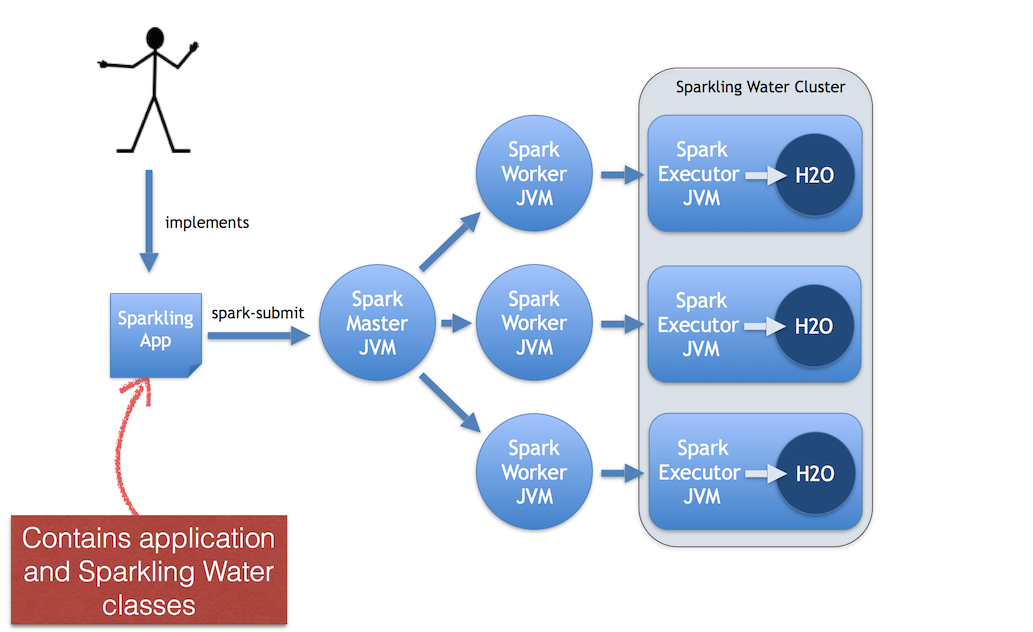
\includegraphics[width=\textwidth]{sw/images/Topology.png}
	\caption{Sparkling Water design. The scenario depicts deployment of Sparkling Water application to standalone Spark cluster.}
\end{figure}


\subsection{Data Sharing between Spark and H2O}

Sparkling Water enables transformation between different types of RDDs and H2O's H2OFrame, and vice versa.

When converting from H2OFrame to RDD, a wrapper is created around the H2O H2OFrame to provide an RDD-like API. In this case, no data is duplicated; instead, the data is served directly from then underlying H2OFrame.

Converting in the opposite direction (from RDD to H2OFrame) introduces data duplication, since it transfers data from RDD storage into H2OFrame. However, data stored in H2OFrame is heavily compressed.

\subsection{Provided Primitives}

\begin{table}
\centering
\begin{tabularx}{\textwidth}{l l p{5.2cm}}
\toprule
Concept & API Representation & Description \\
\midrule
H2O context & \texttt{H2OContext}\footnote{Fullname of class is \texttt{org.apache.spark.h2o.H2OContext}} & Holds
H2O state and provides primitives to publish \texttt{RDD} as \texttt{H2OFrame} and
vice versa. It follows design principles of Spark primitives such as
\texttt{SparkContext} or \texttt{SQLContext} \\  \addlinespace

H2O entry point & \texttt{H2O}\footnote{Fullname of class is \texttt{water.H2Ot}} & Represents the entry point for accessing
H2O services. It holds information about running H2O services including a list of
nodes and the status of distributed K/V datastore. \\  \addlinespace

H2O Frame & \texttt{H2OFrame}\footnote{Fullname of class is \texttt{water.fvec.H2OFrame}} & A data structure that
represents a table of values. The table is column-based and provides column and
row accessors. \\  \addlinespace

H2O Algorithm & package \texttt{hex} & Represents the H2O machine learning
algorithms library, including DeepLearning, GBM, GLM, RandomForest and other
algorithms. \\

\bottomrule
\end{tabularx}
\caption{Sparkling Water primitives}
\label{tab:primitives}
\end{table}


%
% Exposed public Scala API
%
\newpage
\section{Programming API}

\subsection{Scala}



\subsection{Python}



%
% Building standalone applications with Sparklint Water
%
\newpage
\section{Building a Standalone Application}



\newpage
\section{Appendix A: Complete parameter list}


\newpage
\section{Appendix B: References}

\end{document}

